\documentclass[tikz,border=10pt]{standalone}
\usepackage[scaled=0.95]{helvet}
\renewcommand{\familydefault}{\sfdefault}
\usepackage[europeanresistors,americanvoltages]{circuitikz}
\definecolor{TEJNavy}{HTML}{14213D}
\definecolor{TEJBlue}{HTML}{1769AA}
\definecolor{TEJGreen}{HTML}{147D55}
\definecolor{TEJRed}{HTML}{B42318}
\definecolor{TEJGrey}{HTML}{E9EEF5}
\begin{document}
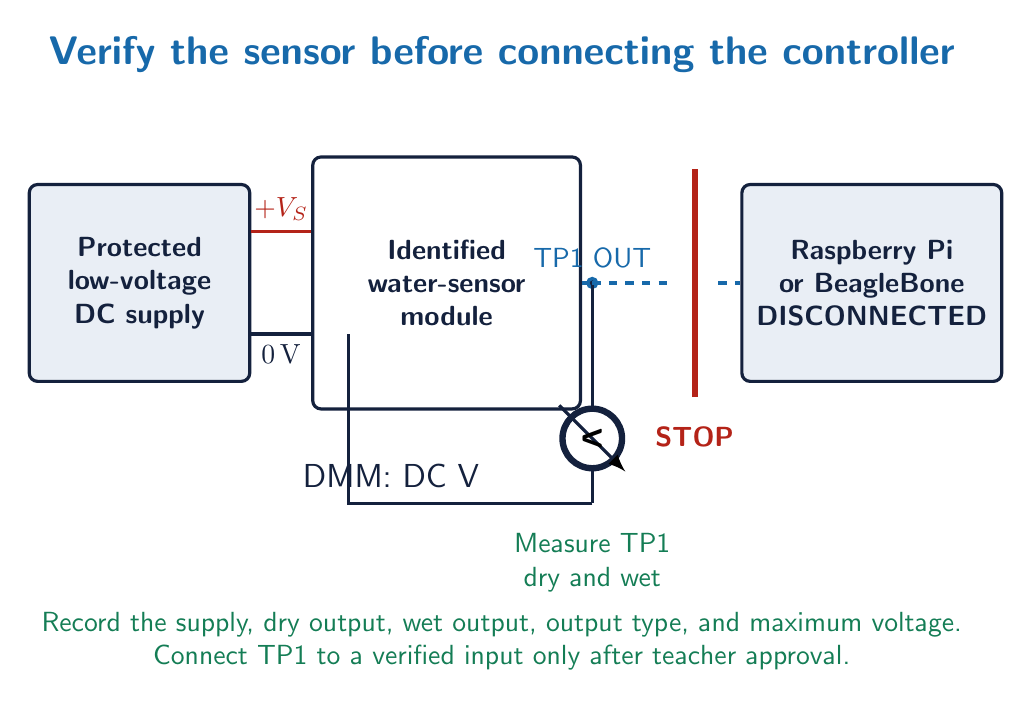
\begin{tikzpicture}[line width=1.15pt,draw=TEJNavy,text=TEJNavy,font=\sffamily]
  \node[font=\bfseries\Large,text=TEJBlue] at (6.2,7.0)
    {Verify the sensor before connecting the controller};

  \node[draw,rounded corners=3pt,fill=TEJGrey,minimum width=2.8cm,minimum height=2.5cm,
    align=center,font=\bfseries] (supply) at (1.6,4.1)
    {Protected\\low-voltage\\DC supply};
  \node[draw,rounded corners=3pt,fill=white,minimum width=3.4cm,minimum height=3.2cm,
    align=center,font=\bfseries] (sensor) at (5.5,4.1)
    {Identified\\water-sensor\\module};
  \node[draw,rounded corners=3pt,fill=TEJGrey,minimum width=3.3cm,minimum height=2.5cm,
    align=center,font=\bfseries] (controller) at (10.9,4.1)
    {Raspberry Pi\\or BeagleBone\\DISCONNECTED};

  \draw[TEJRed,very thick] (supply.east |- 0,4.75) -- node[above] {$+V_S$} (sensor.west |- 0,4.75);
  \draw[TEJNavy,very thick] (supply.east |- 0,3.45) -- node[below] {$0\,\mathrm{V}$} (sensor.west |- 0,3.45);

  \coordinate (tp) at (7.35,4.1);
  \draw[TEJBlue,very thick] (sensor.east) -- (tp) node[circ,label=above:{TP1 OUT}] {};
  \draw (tp) -- ++(0,-1.15) coordinate (vmTop);
  \draw (vmTop) to[voltmeter] ++(0,-1.65) coordinate (vmBottom);
  \draw (vmBottom) -| (4.25,3.45);
  \node[anchor=east,font=\large] at (6.05,1.65) {DMM: DC V};
  \node[TEJGreen,align=center] at (7.35,0.55) {Measure TP1\\dry and wet};

  \draw[TEJRed,line width=2.2pt] (8.65,2.65) -- (8.65,5.55);
  \node[TEJRed,align=center,font=\bfseries] at (8.65,2.15)
    {STOP};
  \draw[TEJBlue,dashed,very thick] (tp) -- (8.35,4.1);
  \draw[TEJBlue,dashed,very thick] (8.95,4.1) -- (controller.west);

  \node[TEJGreen,align=center] at (6.2,-0.45)
    {Record the supply, dry output, wet output, output type, and maximum voltage.\\Connect TP1 to a verified input only after teacher approval.};
\end{tikzpicture}
\end{document}
